\bookchapter{第四十九章：搭建开发环境——Android Studio 与第一个项目}

\chapterintro{工欲善其事，必先利其器。这一章咱们把“厨房”搭好：装好 Android Studio、跑通模拟器、创建人生第一个安卓项目，再把工程结构拆开看个明白。装好环境之后，你会第一次看到自己写的代码变成一个能点的按钮——这个瞬间，很多人会记一辈子。}

\booksection{一、安装 Android Studio}

Android Studio 是谷歌官方的集成开发环境（IDE），免费，功能全家桶：写代码、看界面预览、调试、打包全在里面。安装四步：

\begin{enumerate}
  \item 打开官网 developer.android.com/studio，下载最新稳定版（2026 年 8 月是 Narwhal 之后的版本，Windows/Mac/Linux 都有）；
  \item 运行安装包，一路"下一步"——安装向导会自动带上\textbf{Android SDK}和模拟器组件；
  \item 首次启动时按提示下载 SDK 组件（默认勾选就好，可能需要几分钟和几个 GB 的空间）；
  \item 完成后你会看到欢迎页——恭喜，"厨房"搭好了。
\end{enumerate}

\begin{tcbwarn}{注意：硬件要求心里有数}
Android Studio 是个“吃内存”的家伙：建议\textbf{16GB 内存}起步（8GB 也能跑，但模拟器一开会比较卡）、磁盘预留\textbf{20GB 以上}、CPU 支持虚拟化（BIOS 里开启 VT-x/AMD-V）。如果电脑确实老旧，可以用“真机调试”代替模拟器（本章第四节会讲），体验反而更流畅。

\end{tcbwarn}

\booksection{二、创建你的第一个项目}

在欢迎页点New Project，选\textbf{Empty Activity}模板（最干净的新手模板），然后填三样东西：

\begin{center}
\begin{tabularx}{\linewidth}{|X|X|X|}
\hline
\textbf{配置项} & \textbf{填什么} & \textbf{说明} \tabularnewline
\hline
Name & My First App & 应用名字，显示在手机桌面上 \tabularnewline
Package name & com.example.myfirstapp & 全球唯一标识，习惯是"域名反写"，先按默认 \tabularnewline
Minimum SDK & API 26（Android 8.0） & 最低支持版本，覆盖 95\%+ 设备 \tabularnewline
\hline
\end{tabularx}
\end{center}

\begin{center}\small\color{gray}创建项目要填的三件事\end{center}

点 Finish 后，Android Studio 会用 Gradle 自动下载依赖、构建项目（第一次要等几分钟，之后每次会快很多）。构建完成后，你就有了一个能跑的 App——虽然它还只会显示一行“Hello Android!”。

\begin{tcbinfo}{小贴士：包名的门道}
包名（package name）就像 App 的“身份证号”，全球不能重复，上架后就不能改了。个人练习用\texttt{com.\allowbreak example.\allowbreak xxx}就行；正式产品要换成你自己的域名反写（比如\texttt{com.\allowbreak 你的名字.\allowbreak 应用名}）。别用\texttt{com.\allowbreak example}上架——商店会拒收。

\end{tcbinfo}

\booksection{三、跑起来：模拟器与真机}

代码写好了，得找个“手机”来跑。你有两个选择：

\booksubsection{模拟器（Emulator）}

模拟器是在电脑里虚拟出一台安卓手机。在 Android Studio 里打开Device ManagerCreate Device，挑一台设备（推荐 Pixel 系列） 选一个系统镜像（带 Google APIs 的） 下载 启动。然后点工具栏的绿色三角Run，几秒钟后，“手机”屏幕上就会出现你的 App。

\booksubsection{真机调试（更推荐）}

真机永远是最真实的测试环境——滑动手感、真网络、真传感器，模拟器都比不了。安卓真机调试很简单：

\begin{enumerate}
  \item 手机上打开 [设置] [关于手机]，连点"版本号" 7 次，开启"开发者选项"；
  \item 在 [开发者选项] 里打开\textbf{USB 调试}；
  \item 用数据线连电脑，手机弹窗选"允许 USB 调试"；
  \item 回到 Android Studio，工具栏的设备下拉列表里就会出现你的手机，点 Run。
\end{enumerate}

\textbf{避坑提醒：USB 调试别常开}\par

USB 调试相当于给电脑开了“后门”。在公共场合充电、连接不信任的电脑时，务必关闭 USB 调试，防止别人通过它读取你的数据。平时开发用完就关，养成习惯。

\booksection{四、工程结构拆解：每个文件是干嘛的}

第一次打开项目，左侧的文件树可能让你头晕。别慌，日常开发你 90\% 的时间只跟下面这几个打交道：

\begin{center}
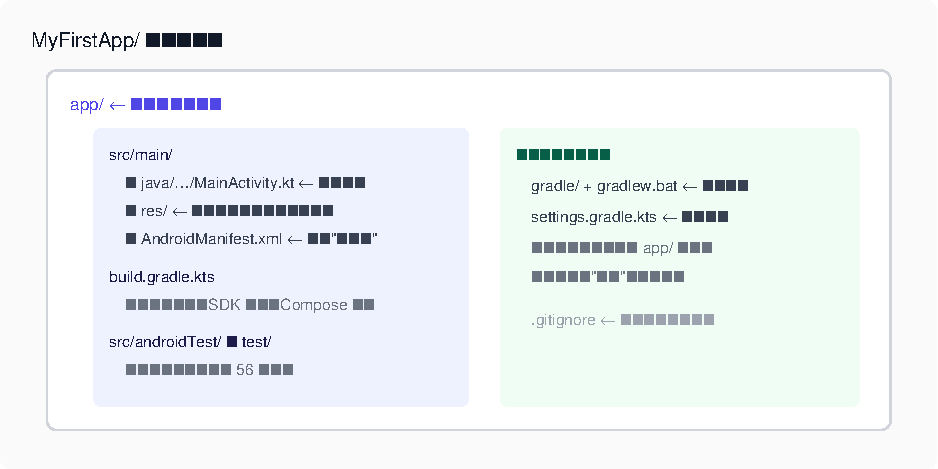
\includegraphics[width=0.92\linewidth]{figures/fig-di-si-shi-jiu-zhang-1}
\\[2pt]\small 图 2：新手必懂的工程结构（口诀：只碰 app/ 目录）
\end{center}

\begin{itemize}
  \item \textbf{MainActivity.kt}：App 的"大门"。用户点开图标，第一个被唤醒的就是它。现在的模板里它负责显示"Hello Android!"。
  \item \textbf{AndroidManifest.xml}：App 的"户口本"——声明这个 App 叫什么、图标是哪个、有哪些页面、要用哪些权限（相机、定位等）。
  \item \textbf{res/ 目录}：资源仓库，存图片、图标、字符串、颜色。把文字放资源文件而不是写死在代码里，是安卓开发的好习惯（换语言、换主题都方便）。
  \item \textbf{build.gradle.kts}：构建配方——声明最低支持版本、依赖哪些库（比如 Compose）。
\end{itemize}

\booksection{五、小试牛刀：把“Hello”换成你的名字}

打开 MainActivity.kt，你会看到 Compose 模板生成的代码。找到\texttt{Text(“Hello Android!”)}这一行，把引号里的字换成你的名字，比如\texttt{Text(“你好，张三！这是我的第一个App”)}，然后按Ctrl+R（Mac 是Cmd+R）重新运行。几秒后，模拟器上就显示了你的名字。

\begin{lstlisting}[language=Kotlin]
setContent {
    MyFirstAppTheme {
        Surface(modifier = Modifier.fillMaxSize()) {
            // v 把这里改成你自己的文字
            Text("你好，张三！这是我的第一个App")
        }
    }
}
\end{lstlisting}

恭喜，你已经完成了一次完整的“改代码 编译 安装 运行”循环。这个循环，就是未来每一天的开发日常。趁热打铁，试着再改点别的：把字号调大、换个颜色——下一章我们就会学到这些“魔法”是怎么来的。

\booksection{六、常见报错急救：新手前两周的“急诊室”}

环境搭建和首次构建阶段，你会大概率遇到下面三种报错。别慌，都有解药：

\begin{center}
\begin{tabularx}{\linewidth}{|X|X|X|}
\hline
\textbf{报错现象} & \textbf{常见原因} & \textbf{解药} \tabularnewline
\hline
Gradle sync failed / 依赖下载慢 & 网络访问仓库不畅 & 给 Gradle 配置国内镜像仓库（阿里云/腾讯云 maven 镜像），网上搜"gradle 国内镜像"照着改 \tabularnewline
SDK 组件缺失 & 安装时跳过了 SDK 下载 & Settings SDK Manager 补装缺失的平台与工具 \tabularnewline
模拟器启动失败 / 黑屏 & 虚拟化未开启、镜像损坏 & BIOS 开 VT-x/AMD-V；删掉模拟器重建；或直接用真机调试 \tabularnewline
\hline
\end{tabularx}
\end{center}

\begin{center}\small\color{gray}新手环境报错急救表\end{center}

\begin{tcbinfo}{小贴士：搜报错的方法论}
报错信息第一行是最有价值的——把它原样复制进搜索引擎，加“android studio”关键词。别搜“我装不上环境怎么办”这种笼统问题，搜“Gradle sync failed: Could not resolve com.android.tools.build”这种具体错误。精确的问题，才有精确的答案。

\end{tcbinfo}

\begin{tcbpractice}{来动手：完成你的"开发仪式感"清单}
(1) 装好 Android Studio 并跑通模拟器；(2) 用真机跑一次自己的 App 并截图留念；(3) 把 Hello 文字改成你的名字；(4) 把项目压缩存个档。做完这四步，你就可以在朋友圈宣布：我也是安卓开发者了（截图为证）。

\end{tcbpractice}

\begin{tcbsummary}{本章小结}
\begin{itemize}
  \item Android Studio = 官方免费 IDE；建议 16GB 内存 + 20GB 磁盘 + 开虚拟化
  \item 新建项目三要素：名字、包名（全球唯一，com.example 别上架）、最低 SDK（API 26 起）
  \item 两种运行方式：模拟器（电脑里虚拟手机）与真机（开 USB 调试，用完记得关）
  \item 工程口诀：只碰 app/ 目录——MainActivity.kt 是大门，Manifest 是户口本，res/ 是资源仓库
  \item 开发日常 = 改代码 Run 看效果，循环往复
\end{itemize}

\end{tcbsummary}
